\documentclass[11pt,a4paper]{article}
\usepackage[T1]{fontenc}\usepackage[utf8]{inputenc}\usepackage[scaled=0.95]{helvet}\renewcommand{\familydefault}{\sfdefault}
\usepackage[a4paper,margin=2.2cm]{geometry}\usepackage{graphicx,booktabs,longtable,amsmath,caption}\usepackage[hidelinks]{hyperref}
\captionsetup{font=small,labelfont=bf}\setlength{\parindent}{0pt}\setlength{\parskip}{0.6em}
\begin{document}
{\LARGE\textbf{How many people cycle rue de Terrebonne in winter, and how often?}}\\[3pt]
{\large Bicycle counts on four sensors, a frequency distribution, and the APC-NDG survey in context}\\[4pt]
{\small Terrebonne-open-sources, 2026-11-07. Author: a resident of Côte-des-Neiges--Notre-Dame-de-Grâce (see the repository\textquoteright{}s « About the author »). Data: borough loop counter (access requests 2026-300 and 2026-581), the author\textquoteright{}s Telraam sensors (counts: Telraam), City open data (CC-BY 4.0), ECCC. Code, tables and figures: \url{https://openmobilitydata.github.io/Terrebonne-open-sources/2026-winter-counts-user-frequency/}.}

\section*{Abstract}
The borough\textquoteright{}s winter figures for rue de Terrebonne are passage counts at one point, Kensington, and the public debate has read them as numbers of people. This note asks what the available counts can and cannot say about the number of individuals who cycle the street in winter and how often, and uses the answer to place the APC-NDG survey of October--November 2026 (87 respondents cycled on Terrebonne last winter, 36 at least weekly) in context. Four sensors overlap in the winter of 2025--26: the borough\textquoteright{}s loop at Kensington, two Telraam sensors at King Edward and Draper, and the City\textquoteright{}s detector at Girouard (westbound only); two Miovision one-day counts of 2024 and 2025 give snapshots. From December~1, 2025 to February~28, 2026 the loop recorded 3,232 passages (41.8 per weekday, 20.5 per weekend day); 53\,\% of weekday passages are in matched morning--evening round trips, about 11 per weekday; 41\,\% of passages are in darkness. Winter traffic concentrates toward the east end: on dry days Draper carries 1.33 and King Edward 0.57 times the Kensington count, and the City\textquoteright{}s westbound count at Girouard is 1.58 times the loop\textquoteright{}s. The Telraam-to-loop ratio rises by 50--60\,\% on days with snowfall, a discrepancy whose cause (over-detection, or cyclists leaving the snowed-in lane for the roadway where the loop cannot see them) the data do not settle. A model-free bound puts at least 154 distinct cyclists on the street at King Edward on 2026-03-09 and at least 65 at Kensington on 2026-03-30. A negative-binomial mixture of three frequency bands fitted to the daily counts and the matched pairs shows what a single counter identifies: the passages produced by frequent riders and their round trips, but not the number of people behind them without an assumption on how often each rides; across four template variants the frequent core at Kensington lies between 11 and 85 people and the occasional tail between 25 and 292. On any reading, the 87 individuals found by a voluntary survey are a floor under the winter riding population, not a measure of it, and the passages they report are consistent with the count.

\tableofcontents

\section{Question}
Two units run through the discussion of the winter layout adopted by the borough council on November 2, 2026 (file 1266880005). The counters count \emph{passages}: one bicycle crossing one point in one direction. The survey counts \emph{people}. Exposure to risk and the use made of the lane accrue per passage; representation and the reach of a measure are counted in persons. Neither unit converts into the other without an assumption about how often each person rides and how many times a trip crosses the counting point. This note states those assumptions explicitly and asks three questions: what the structure of the counts (hour of day, day of week, weather, several points along the street) says about the mix of frequent and occasional riders; what bounds and estimates on the number of individuals follow, and with what uncertainty; and how the survey\textquoteright{}s figures, 87 respondents who cycled on Terrebonne last winter and 36 at least weekly, sit against them. The survey figures used are those of the public filing of November 2, 2026; its finer frequency categories are not used here.

\section{Data}
\subsection{Sensors}
\begin{itemize}
\item \textbf{Kensington loop} (borough, Eco-Counter ZELT EVO, 45.47022~N, 73.63204~W): hourly counts by direction (eastbound \emph{IN\_est}, westbound \emph{OUT\_ouest}) from July 26, 2025 to May 11, 2026 (request 2026-300), daily totals to August 31, 2026 (request 2026-581). The westbound channel is degraded from about March 1, 2026 (the borough engineering division\textquoteright{}s reply of October 15, 2026, and the supplier\textquoteright{}s of October 21): the analyses below use December~1, 2025 to February~28, 2026 as the \emph{core} period, and December~1 to March~31 (the proposed conversion window) only for totals, which are then lower bounds.
\item \textbf{King Edward} (Telraam S2, segment 13374, west of Cavendish) and \textbf{Draper} (segment 13690, east of Kensington), installed by the author in August and September 2024: hourly counts of bicycles in two directions (A$>$B, B$>$A) with an uptime per hour; a camera sensor that counts in daylight only. Draper stopped on January 24, 2026; King Edward ran to May 4, 2026. The counts are Telraam\textquoteright{}s under its terms of use; only aggregates are published here.
\item \textbf{Girouard} (City detector det-00118, open data « Compteurs cyclistes permanents »): daily and hourly volumes from October 23, 2025; instance 01 is Terrebonne westbound (the only Terrebonne direction reported), instances 02--03 are Girouard itself.
\item \textbf{Miovision one-day counts} (request 2026-581, by approach in request 2026-634): September 19, 2024 and January 29, 2025 at Grand and at Cavendish, six peak hours and twelve hours.
\item \textbf{Weather}: ECCC daily, Montréal-Trudeau (7025251): snowfall, mean and minimum temperature, snow on the ground. \textbf{Daylight}: sunrise and sunset computed (NOAA algorithm) for the site.
\end{itemize}
\subsection{Coverage}
Winter 1 (December 1, 2024 to March 31, 2025) has the two Telraam sensors only; winter 2 (December 1, 2025 to March 31, 2026) has all four points, Draper to January 23. A Telraam day is valid with at least 8 reported hours and 6~h of uptime (the convention of the Terrebonne-telraam repository).
{\small\begin{longtable}{@{}llllll@{}}\toprule Sensor & winter & valid days & first & last & passages\\ \midrule
Kensington loop (borough) & W2 2025-26 & 121 of 121 & 2025-12-01 & 2026-03-31 & 4,891 \\
King Edward (Telraam) & W1 2024-25 & 119 of 121 & 2024-12-01 & 2025-03-31 & 5,422 \\
King Edward (Telraam) & W2 2025-26 & 68 of 121 & 2025-12-01 & 2026-03-31 & 3,268 \\
Draper (Telraam) & W1 2024-25 & 120 of 121 & 2024-12-01 & 2025-03-31 & 5,978 \\
Draper (Telraam) & W2 2025-26 & 53 of 121 & 2025-12-01 & 2026-01-24 & 1,752 \\
Girouard WB (City det-00118-01) & W2 2025-26 & 115 of 121 & 2025-12-01 & 2026-03-31 & 3,150 \\
\bottomrule\end{longtable}}
\begin{figure}[htbp]\centering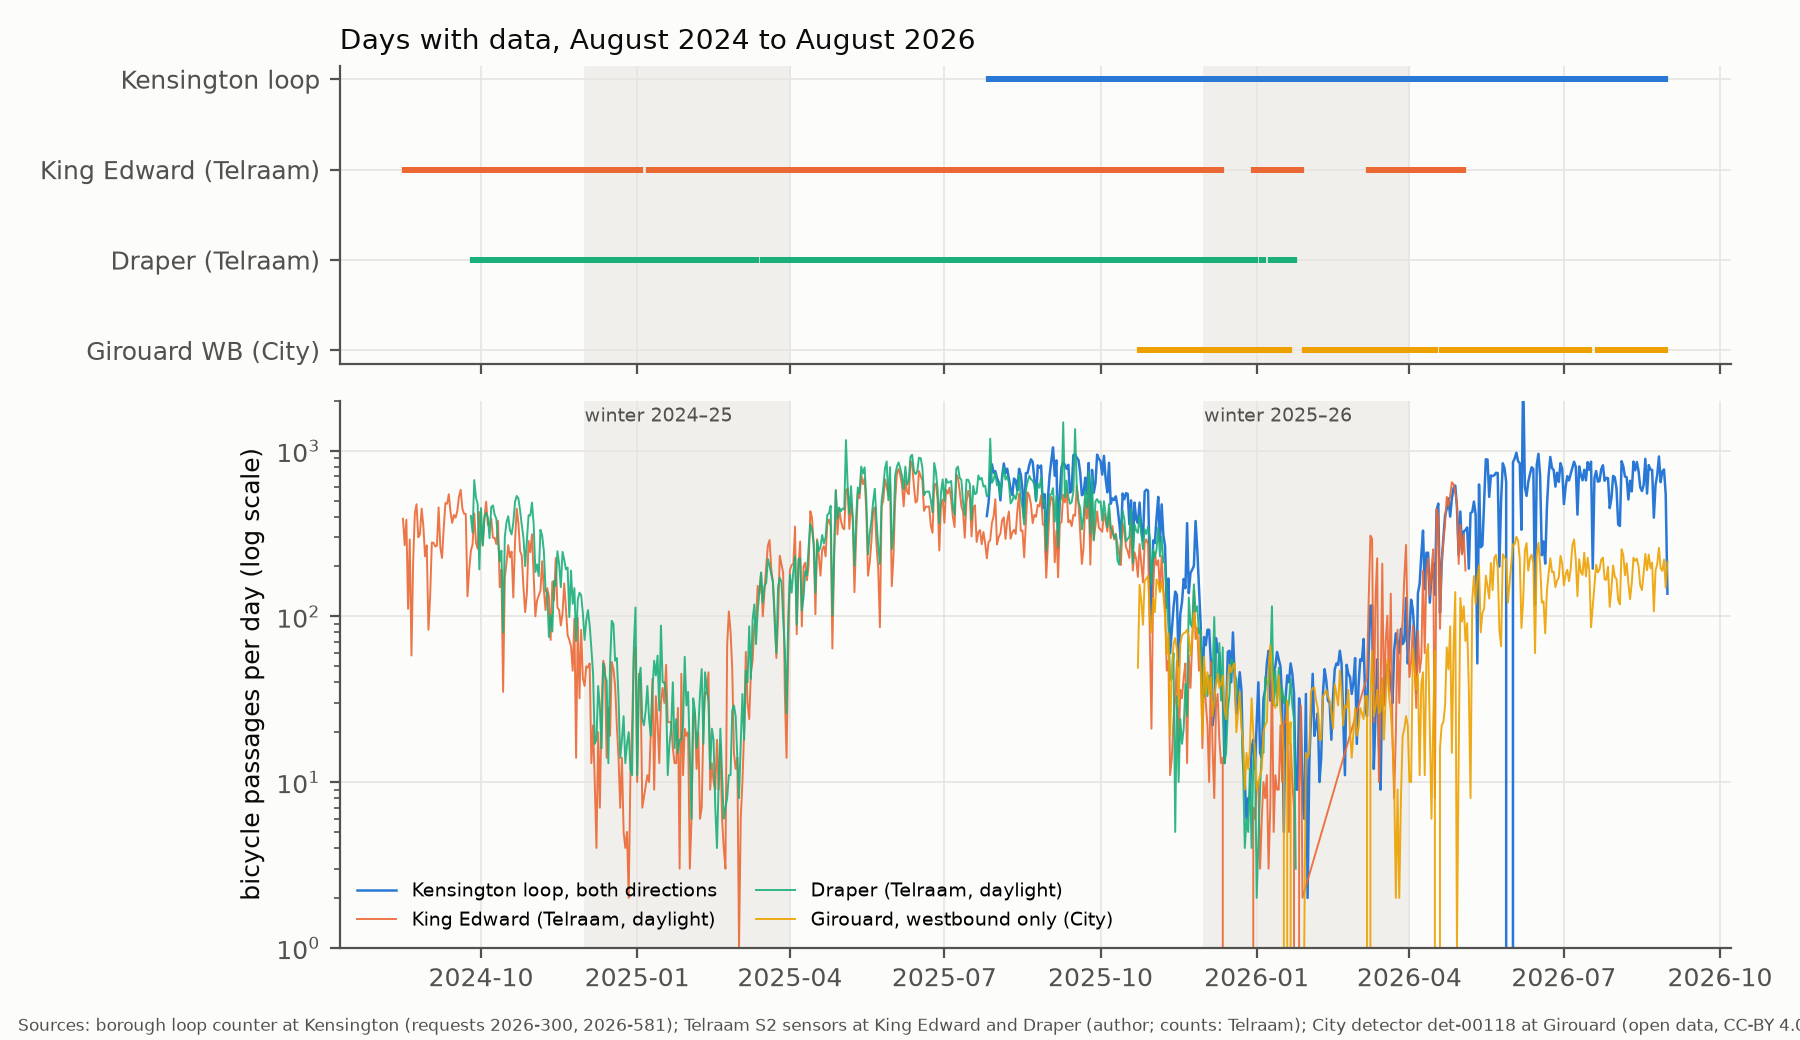
\includegraphics[width=1.0\textwidth]{figures/coverage_and_series_en.png}\caption{Days with data on each sensor (top) and daily passages (bottom, log scale). Telraam: daylight hours; Girouard: westbound only.}\label{fig:coverage_and_series}\end{figure}

\section{Methods}
\subsection{Matching the sensors}
Telraam and loop are compared on the same clock hours of the same days, 8--16~h, with Telraam uptime of at least 0.7 in the hour; the ratio of summed passages is computed by month, by hour of day over a season, and separately for days with and without snowfall (ECCC $\geq 2.5$~cm). A ratio that is flat across the hours of the day indicates a real difference in traffic between the two points; a ratio that falls at dawn and dusk indicates the camera\textquoteright{}s detection loss. The Telraam directions were mapped to eastbound and westbound by correlating hourly A$>$B and B$>$A with the loop\textquoteright{}s two channels over September--October 2025. Girouard westbound is compared with the loop\textquoteright{}s westbound channel on common days with at least 20 reported hours.
\subsection{The structure of the winter at Kensington}
For every day of the core period: passages by direction and hour; the number of \emph{matched round trips}, defined as $\min(\text{EB}_{6\text{--}10\text{h}}, \text{WB}_{15\text{--}20\text{h}}) + \min(\text{WB}_{6\text{--}10\text{h}}, \text{EB}_{15\text{--}20\text{h}})$, a lower bound on the number of people who crossed the point outbound in the morning and back in the evening; the share of passages before sunrise or after sunset; the day type (weekday, weekend, holiday period December 22 to January 4) and the weather class (\emph{harsh} = snowfall $\geq 2.5$~cm or mean temperature $\leq -10\,^\circ$C). A negative-binomial regression of the daily total on these variables gives the size of each effect with a standard error.
\subsection{Model-free bounds on distinct users}
If no person crosses a point more than $m$ times in a day, the number of distinct people who rode on a given day is at least the day\textquoteright{}s count divided by $m$; the largest day of the winter at each point therefore gives a lower bound on the number of individuals who cycled the street that winter, with no other assumption. Both $m = 2$ (every passage half of a round trip) and $m = 4$ are reported.
\subsection{A frequency-band model}
Let $Y_d$ be the passages on day $d$ and $P_d$ the matched round trips on weekday $d$. Three bands of riders are defined by \emph{templates}: for band $b$, the probability $p_b(d)$ of riding on a day of a given type and weather, the passages per riding day $c_b$ (2 for a round trip through the point, less when trips are one-way), and the share $\pi_b$ of riding days that produce a matched pair. With $N_b$ people in band $b$,
\[ Y_d \sim \mathrm{NB}\Big(\mu_d = \sum_b N_b\, p_b(d)\, c_b,\ r_Y\Big), \qquad P_d \sim \mathrm{NB}\Big(\sum_b N_b\, p_b(d)\, \pi_b,\ r_P\Big), \]
and $N_b$ and the dispersions are estimated by maximum likelihood on the core period. Each $N_b$, and the sum $N_\text{daily} + N_\text{regular}$ (\emph{frequent}), receives a 95\,\% profile-likelihood interval. Because the templates, not the data, define what \emph{frequent} and \emph{occasional} mean, the fit is repeated with four template sets:
\begin{itemize}
\item \textbf{base}: daily: rides 80 \% of mild weekdays, 70 \% of harsh weekdays (snow >= 2.5 cm or mean temperature <= -10 C), 30 \% of holiday weekdays (Dec 22 to Jan 4), 5 \% of weekend days (3 \% harsh); 2 passages per riding day, 80 \% of them as matched AM/PM pairs. regular: 35 \% / 25 \% / 12 \% / 15 \% (8 \%); 2 passages; 60 \% paired. occasional: 10 \% / 6 \% / 6 \% / 12 \% (6 \%); 1.5 passages; 30 \% paired
\item \textbf{more one-way trips}: as base, but fewer passages per riding day (daily 1.8, regular 1.6, occasional 1.2: more one-way trips through the point) and fewer matched pairs
\item \textbf{tail more weather-sensitive}: as base, but the regular and occasional bands drop more on harsh days (regular 12 \%, occasional 2 \%) and the daily band less (75 \%)
\item \textbf{survey categories literal}: riding days taken from the survey categories at face value: most weekdays = 90 \% of weekdays; one to three days a week = 2 of 5 weekdays; a few times a month = 2.5 days a month spread over all days; weather and holiday factors in the same proportions as base
\end{itemize}
The model is deliberately simple. Its purpose is to show which quantities a single counter determines and which it does not.
\subsection{From one point to the street, and the survey}
Passages at King Edward, Draper and Girouard relative to Kensington, on dry days, bound the number of trips that cross at least one point: between the largest point and the sum of the points, in units of the Kensington count. For the survey, the passages its respondents would have produced at one point are computed under stated ranges of riding days per winter and passages per riding day, and compared with the count; the modelled bands give the share of each kind of rider the survey reached.

\section{Results}
\subsection{The winter at Kensington}
From December~1, 2025 to February~28, 2026 (90 days) the loop counted 3,232 passages (1,626 eastbound, 1,606 westbound). Weekdays average 41.8 passages (median 41, 10th--90th percentiles 17--62, range 6--83); weekend days 20.5 (median 15). Mild weekdays average 50.6 (n = 28), harsh weekdays 40.1 (n = 27, minimum 6), holiday weekdays 22.0. Matched round trips average 11.0 per weekday (10th--90th percentiles 1--20) and account for 53\,\% of weekday passages; 41\,\% of all passages occur before sunrise or after sunset. Over the whole window December~1 to March~31 the loop counted 4,891 passages, with no day below 2 and 60 days of 40 or more; the largest day, 2026-03-30, had 129 (westbound channel degraded in March: a lower bound).
\begin{figure}[htbp]\centering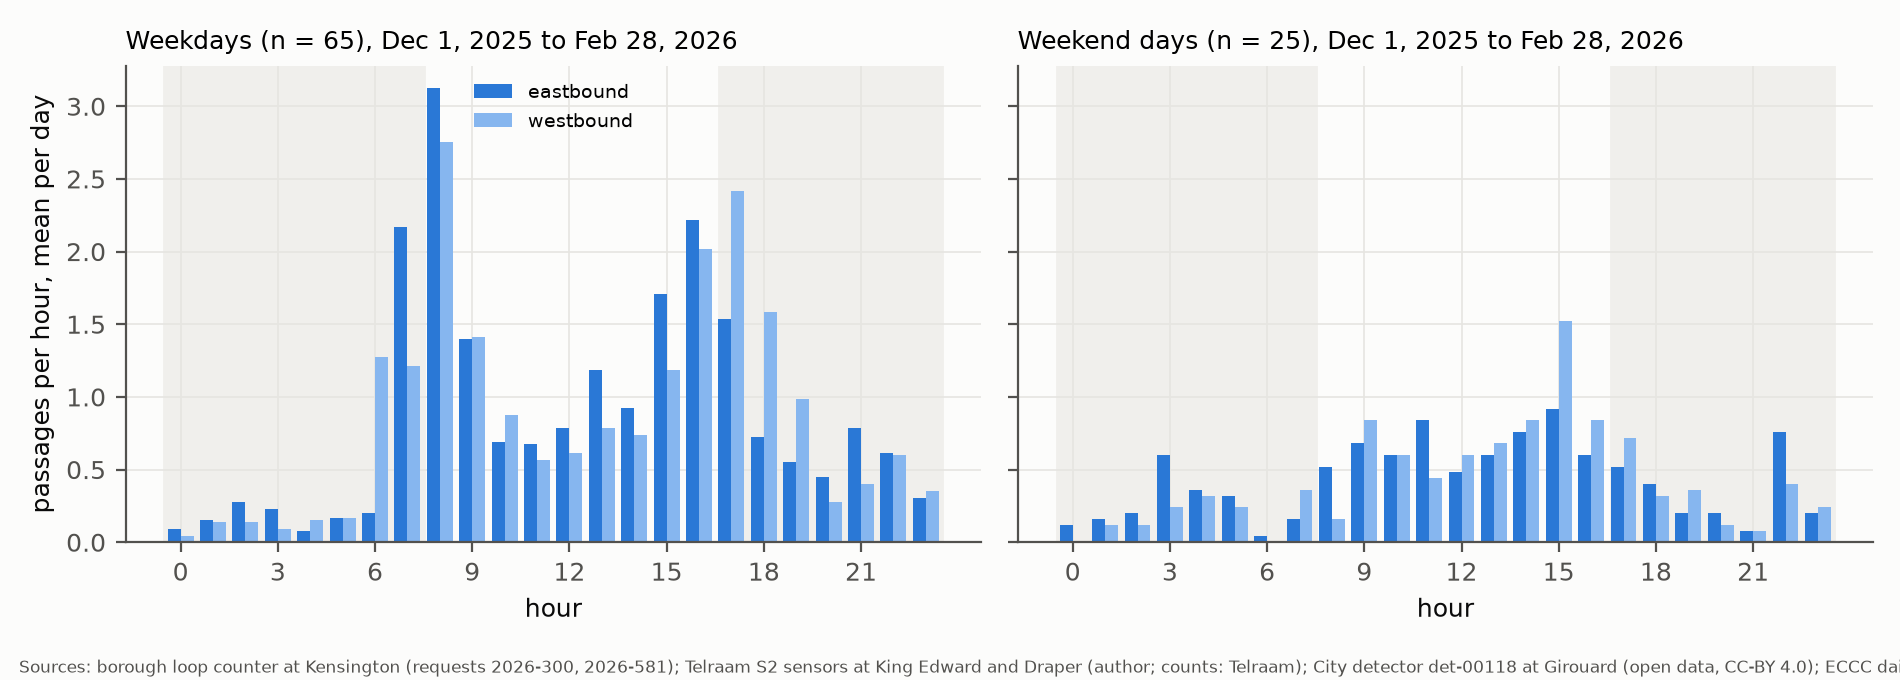
\includegraphics[width=1.0\textwidth]{figures/kensington_hourly_profile_en.png}\caption{Mean passages per hour by direction, weekdays and weekend days, December 1, 2025 to February 28, 2026; shaded = before sunrise and after sunset on January 15.}\label{fig:kensington_hourly_profile}\end{figure}
\begin{figure}[htbp]\centering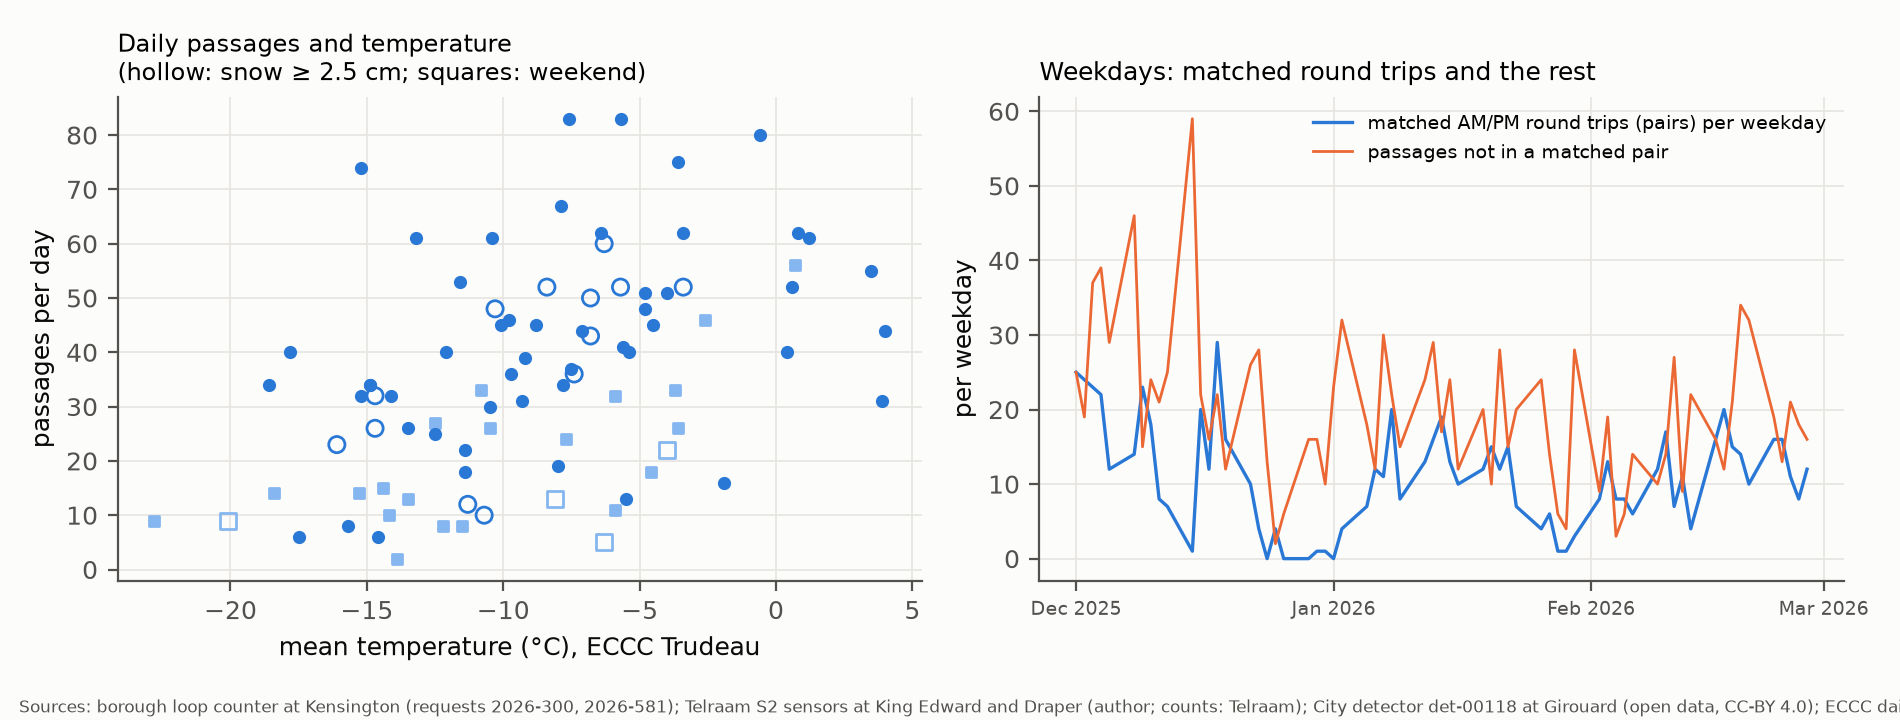
\includegraphics[width=1.0\textwidth]{figures/kensington_weather_pairs_en.png}\caption{Left: daily passages against mean temperature. Right: matched morning--evening round trips per weekday and the passages outside them.}\label{fig:kensington_weather_pairs}\end{figure}

The negative-binomial regression (Table~\ref{tab:nb}; n = 90 days, dispersion $r$ = 8.51) puts the weekend at -49 \% and the holiday period at -41 \% relative to an ordinary weekday; each degree of mean temperature adds +3 \%, each centimetre of snow on the ground removes 2 \%; the day\textquoteright{}s own snowfall has no separate effect once snow on the ground and temperature are in; daylight hours and the time trend are confounded over a ninety-day window and should be read together. The lag-1 autocorrelation of the weekday residuals is 0.182: day-to-day persistence beyond the weather is weak.
\begin{table}[htbp]\centering\small\caption{Negative-binomial regression of daily passages at Kensington, core period. Coefficients per unit of the raw variable; standard errors approximate (BFGS inverse Hessian).}\label{tab:nb}
\begin{tabular}{@{}lrrl@{}}\toprule term & coefficient & s.e. & effect\\ \midrule
intercept & 3.469 & 0.044 & mean on an average day: 32.1 passages \\
weekend & -0.6667 & 0.1066 & -49 \% \\
holiday & -0.5283 & 0.1635 & -41 \% \\
snow cm & -0.0005 & 0.0181 & -0 \% per unit \\
tmean c & 0.033 & 0.009 & +3 \% per unit \\
snow on ground cm & -0.0223 & 0.0134 & -2 \% per unit \\
daylight h & 0.4187 & 0.1596 & +52 \% per unit \\
days since dec1 & -0.0126 & 0.0045 & -1 \% per unit \\
\bottomrule\end{tabular}\end{table}

\subsection{The other points}
On matched daylight hours King Edward counts 0.65 times the loop in September--October 2025 and 0.60 times in the winter core; Draper 0.76 in autumn and 1.46 in winter. The ratio by hour of day (Figure~\ref{fig:cross_sensor_ratios}) is roughly flat for King Edward in both seasons and falls only at the edges of daylight, as expected of a camera; Draper\textquoteright{}s winter ratio is above one through the day. The Telraam direction split is not recoverable from the data: the correlations of A$>$B with the loop\textquoteright{}s two channels differ by less than 0.1 at both sensors (King Edward 0.578/0.606, Draper 0.614/0.789), so only totals are used. The City\textquoteright{}s westbound count at Girouard is 0.86 times the loop\textquoteright{}s westbound channel in November and 1.59, 1.39 and 1.71 times in December, January and February (Table~\ref{tab:gir}): within one pair of instruments, the east end gains relative to Kensington when winter comes.

\textbf{Snow days.} Table~\ref{tab:wx} splits the winter ratios by weather. On days without snowfall King Edward is at 0.57 and Draper at 1.33 of the loop; on days with 2.5~cm or more they rise to 0.88 and 2.13. The two instruments diverge on snow days by 50--60\,\%, in the same direction at both Telraam sites. Two explanations fit: the camera over-detects on snow days (snow-clearing equipment, pedestrians on the roadway), or cyclists leave the snowed-in lane for the roadway, where an inductive loop placed in the lane cannot see them, so that the loop under-counts. The data do not separate them; the dry-day ratios are used below, and the loop\textquoteright{}s snow-day counts should be read as possibly low.
\begin{table}[htbp]\centering\small\caption{Telraam against the loop on matched hours (8--16~h, uptime $\geq 0.7$), winter core (Draper to January 23), by weather.}\label{tab:wx}
\begin{tabular}{@{}llrrrrr@{}}\toprule sensor & days & n days & matched hours & Telraam & Kensington & ratio\\ \midrule
King Edward & no snow & 15 & 129 & 185 & 322 & 0.575 \\
King Edward & snow ge 2.5cm & 13 & 117 & 204 & 231 & 0.883 \\
King Edward & mild & 16 & 141 & 203 & 442 & 0.459 \\
King Edward & harsh & 27 & 229 & 351 & 480 & 0.731 \\
Draper & no snow & 23 & 187 & 611 & 459 & 1.331 \\
Draper & snow ge 2.5cm & 12 & 96 & 405 & 190 & 2.132 \\
Draper & mild & 24 & 188 & 747 & 582 & 1.284 \\
Draper & harsh & 28 & 222 & 789 & 467 & 1.69 \\
\bottomrule\end{tabular}\end{table}
\begin{table}[htbp]\centering\small\caption{Girouard westbound (City det-00118-01) against the loop\textquoteright{}s westbound channel, common days with $\geq 20$ reported hours.}\label{tab:gir}
\begin{tabular}{@{}lrrrr@{}}\toprule month & days & Girouard WB & Kensington WB & ratio\\ \midrule
2025-11 & 30 & 2,535 & 2,930 & 0.865 \\
2025-12 & 31 & 1,007 & 635 & 1.586 \\
2026-01 & 21 & 518 & 372 & 1.392 \\
2026-02 & 26 & 780 & 455 & 1.714 \\
\bottomrule\end{tabular}\end{table}
\begin{figure}[htbp]\centering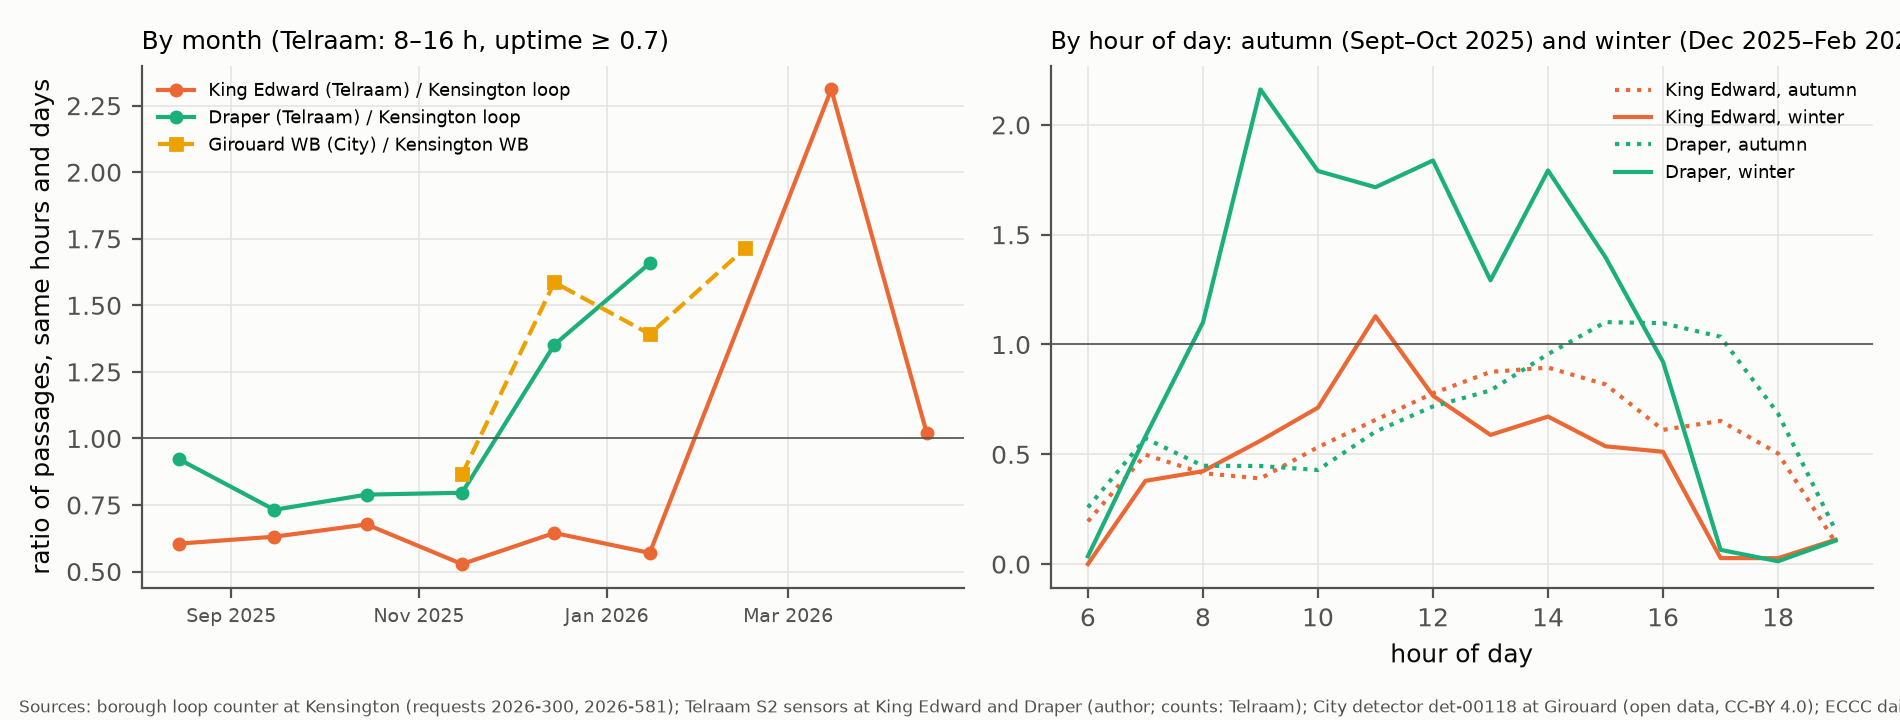
\includegraphics[width=1.0\textwidth]{figures/cross_sensor_ratios_en.png}\caption{Left: ratio of passages to the Kensington loop by month (Telraam on matched daylight hours; Girouard westbound on common days). Right: the same ratio by hour of day, autumn and winter.}\label{fig:cross_sensor_ratios}\end{figure}

\textbf{Two snapshots.} On September 19, 2024 the Miovision camera at Grand counted 667 bicycles on the Terrebonne axis over twelve hours and the one at Cavendish 503; the Telraam at King Edward counted 572 over the same hours (Draper not yet installed). On January 29, 2025, a day with 7.4~cm of snow and a mean temperature of -11.5$\,^\circ$C, Grand counted 12 on the axis over twelve hours (8 on the eastbound approach and 0 on the westbound approach in the six peak hours: the « 8 » of the borough\textquoteright{}s deck), Cavendish 18, King Edward 21 and Draper 57 (11 of 12 hours reported). The Draper figure is a snow-day Telraam count and carries the discrepancy just described; the other three are consistent with one another and with the winter gradient. On that day the eight eastbound passages at Grand had no westbound counterpart in the count window, so they cannot be read as four people going out and coming back through that point in those hours.
\begin{figure}[htbp]\centering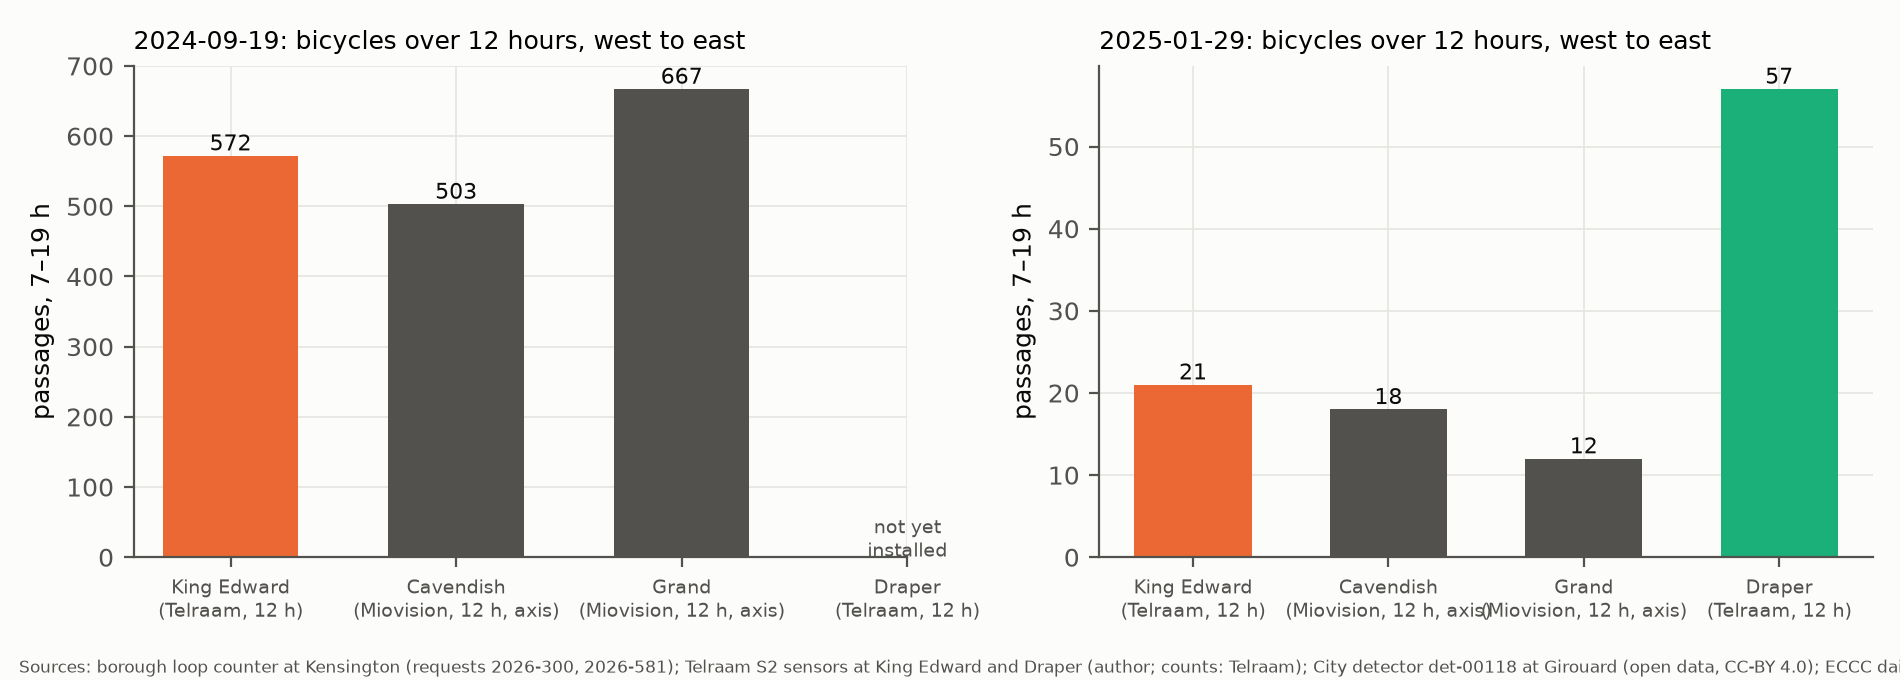
\includegraphics[width=1.0\textwidth]{figures/snapshot_days_en.png}\caption{The two Miovision days with the Telraam sensors on the same hours (7--19~h).}\label{fig:snapshot_days}\end{figure}

\subsection{Bounds on distinct users}
The largest day at each point gives a floor under the number of individuals who cycled the street in the winter of 2025--26 (Table~\ref{tab:bounds}). At King Edward, 2026-03-09 (a Monday, no snowfall) had 307 passages in daylight: at least 154 people if no one passed more than twice, 77 if no one passed more than four times, on a sensor that counts about 0.6 of the loop on comparable days. At Kensington the largest day of the window, 2026-03-30, gives at least 65 with the westbound channel degraded; within the core period, 2025-12-03 gives at least 42. Draper\textquoteright{}s largest day (2026-01-10, 115) fell on a day with 7.8~cm of snow and is not used.
\begin{table}[htbp]\centering\small\caption{Largest day of the winter window at each point and the implied floor on distinct cyclists.}\label{tab:bounds}
\begin{tabular}{@{}llrrrl@{}}\toprule point & date & passages & people, $m=2$ & people, $m=4$ & note\\ \midrule
Kensington loop & 2026-03-30 & 129 & 65 & 33 & westbound channel degraded\\
Kensington loop, core & 2025-12-03 & 83 & 42 & 21 & both channels sound\\
King Edward (Telraam) & 2026-03-09 & 307 & 154 & 77 & daylight; no snowfall\\
Draper (Telraam) & 2026-01-10 & 115 & -- & -- & snow day, not used\\
Girouard WB (City) & 2026-01-09 & 67 & 34 & 17 & one direction\\
\bottomrule\end{tabular}\end{table}

\subsection{The frequency bands}
Table~\ref{tab:bands} gives the fitted number of people in each band at Kensington for the four template sets, with the profile-likelihood intervals, the share of passages produced by the frequent bands and the fitted total against the observed 3,232. Figure~\ref{fig:band_fit} shows the fit by day type and the profile curves for the base templates.
\begin{table}[htbp]\centering\small\caption{Frequency-band model at Kensington, December 1, 2025 to February 28, 2026: people per band (95\,\% profile interval), by template set.}\label{tab:bands}
\begin{tabular}{@{}lllllrr@{}}\toprule templates & most weekdays & 1--3 days a week & frequent (both) & a few times a month & share of passages, frequent & fitted total\\ \midrule
base & 0 (0--10) & 61 (22--69) & \textbf{61} (32--70) & 66 (25--128) & 78\,\% & 3,151 \\
more one-way trips & 0 (0--12) & 73 (16--85) & \textbf{73} (29--85) & 88 (37--175) & 76\,\% & 3,118 \\
tail more weather-sensitive & 15 (10--16) & 0 (0--37) & \textbf{15} (12--48) & 253 (158--292) & 41\,\% & 3,380 \\
survey categories literal & 0 (0--11) & 41 (0--46) & \textbf{41} (11--48) & 173 (128--238) & 56\,\% & 3,225 \\
\bottomrule\end{tabular}\end{table}
\begin{figure}[htbp]\centering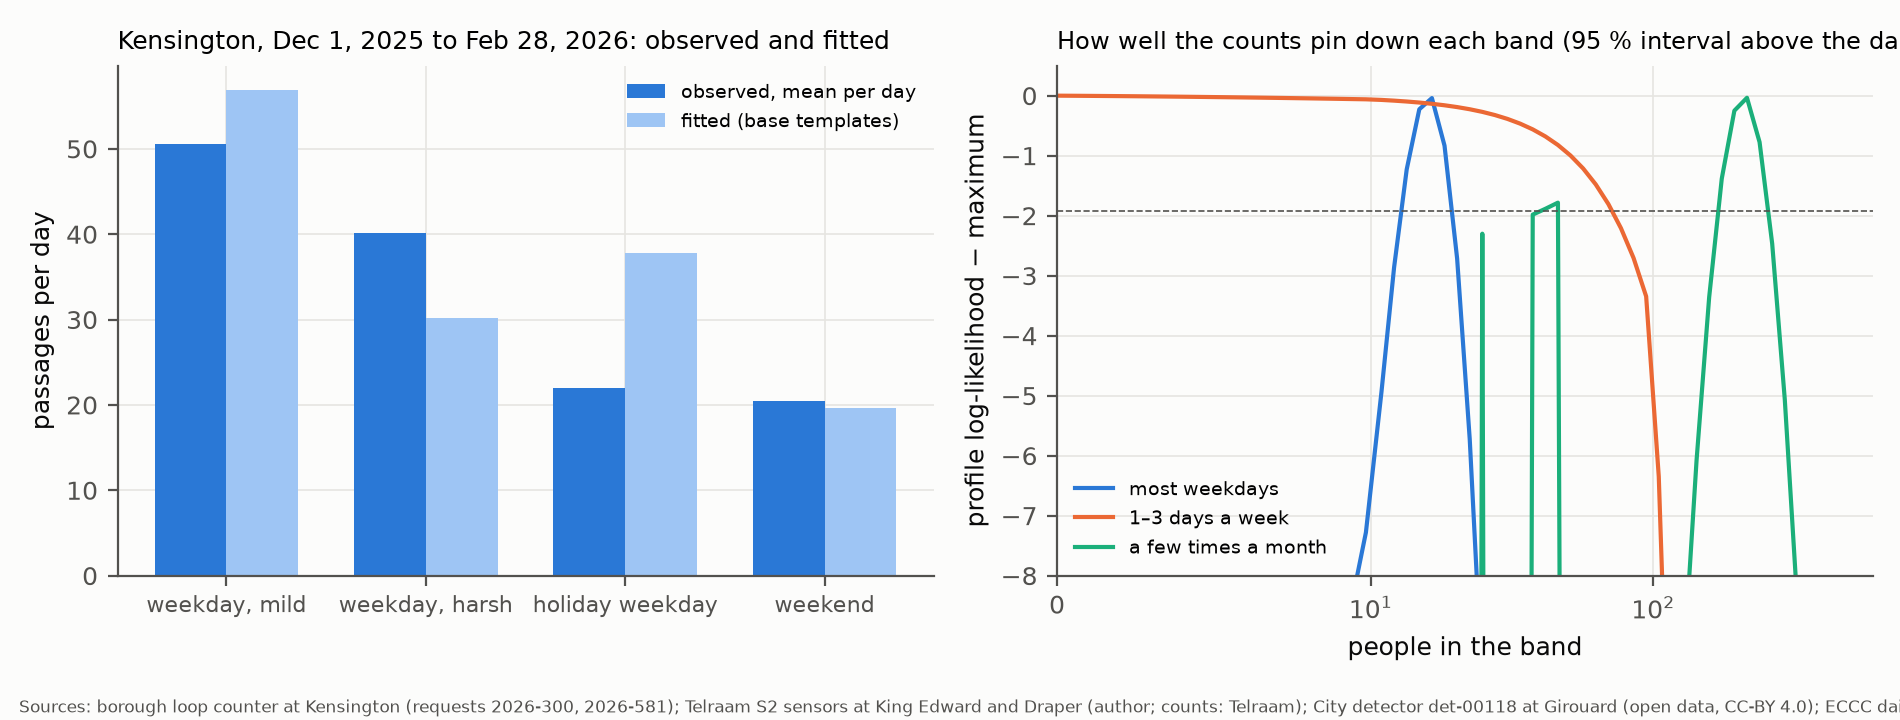
\includegraphics[width=1.0\textwidth]{figures/band_fit_en.png}\caption{Left: observed and fitted mean passages by day type (base templates). Right: profile log-likelihood for each band and for the frequent core; the 95\,\% interval is the range above the dashed line.}\label{fig:band_fit}\end{figure}

Three things are stable across the template sets. First, the frequent core is small in number and large in passages: between 11 and 85 people produce 41--78\,\% of the winter passages at this point. Second, the split of that core between daily and one-to-three-days-a-week riders is not identified by the counts: the two bands trade against each other along a ridge of the likelihood, and the fitted split moves from all-daily to all-regular with changes in the templates that the data cannot reject. Third, the occasional tail is large in people and uncertain: 25 to 292 across the fits, because a given volume of tail passages can come from fewer people riding more often or more people riding less. Table~\ref{tab:tail} makes that dependence explicit for the base fit.
\begin{table}[htbp]\centering\small\caption{The occasional tail of the base fit (688 passages) as a number of people, for a range of rides per winter per person (1.5 passages per ride).}\label{tab:tail}
\begin{tabular}{@{}rrr@{}}\toprule rides per winter & passages per person & people\\ \midrule
2 & 3.0 & 229 \\
3 & 4.5 & 153 \\
4 & 6.0 & 115 \\
6 & 9.0 & 76 \\
8 & 12.0 & 57 \\
12 & 18.0 & 38 \\
\bottomrule\end{tabular}\end{table}

\subsection{From Kensington to the street}
On dry days King Edward carries 0.57, Draper 1.33 and Girouard westbound 1.58 times the corresponding Kensington count. Trips that cross at least one of the four points number between 1.58 and 4.48 times the Kensington count, the lower figure if every trip crosses every point, the upper if no trip crosses two. The truth is between: trips from the west end to Villa-Maria cross all four, trips within Monkland Village cross one. Any figure for people on the street as a whole is the Kensington figure scaled by a factor in that range, and the uncertainty of the factor is of the same order as the uncertainty of the band model.

Year over year, on common valid calendar dates, King Edward counted 0.77 and Draper 0.81 times in the winter of 2025--26 what they counted in 2024--25 (66 and 53 days): the winter studied here was not the busier of the two.

\subsection{The survey in context}
The survey\textquoteright{}s public filing reports 87 respondents who cycled on Terrebonne in the winter of 2025--26, 36 of them at least weekly, among 161 respondents kept. Table~\ref{tab:sv} gives the passages they would have produced at one point if every trip crossed it, for stated ranges of riding days and passages per riding day; Figure~\ref{fig:survey_vs_count} compares them with the count.
\begin{table}[htbp]\centering\small\caption{Passages implied by the survey\textquoteright{}s 87 winter cyclists at one point, December 1 to March 31 (17.3 weeks), under stated assumptions.}\label{tab:sv}
\begin{tabular}{@{}llrrrr@{}}\toprule band & riding days per winter & passages per riding day & low & central & high\\ \midrule
at least weekly (36) & 17--86 (central 43) & 1.0 & 622 & 1,556 & 3,111 \\
at least weekly (36) & 17--86 (central 43) & 1.5 & 933 & 2,334 & 4,667 \\
at least weekly (36) & 17--86 (central 43) & 2.0 & 1,245 & 3,111 & 6,223 \\
less than weekly (51) & 4--12 (central 8) & 1.0 & 204 & 408 & 612 \\
less than weekly (51) & 4--12 (central 8) & 1.5 & 306 & 612 & 918 \\
less than weekly (51) & 4--12 (central 8) & 2.0 & 408 & 816 & 1,224 \\

\bottomrule\end{tabular}\end{table}
\begin{figure}[htbp]\centering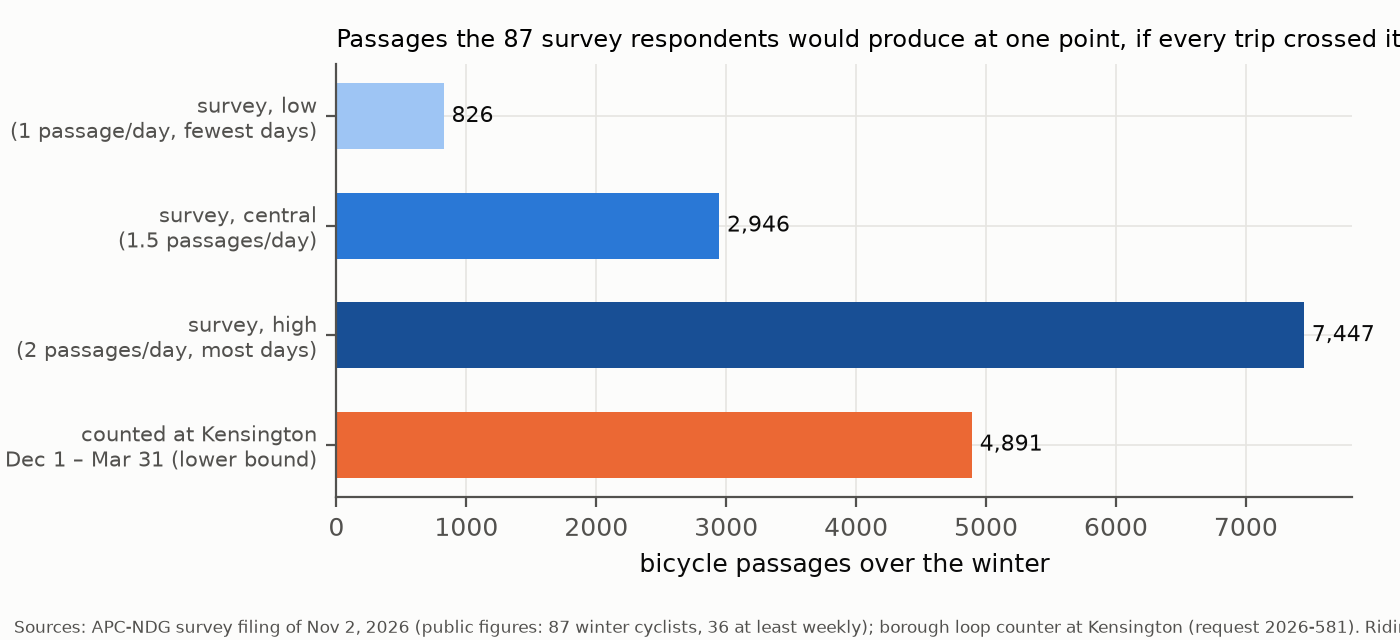
\includegraphics[width=0.85\textwidth]{figures/survey_vs_count_en.png}\label{fig:survey_vs_count}\end{figure}

Under central assumptions the 87 account for 2,946 passages, 60\,\% of the 4,891 counted at Kensington over the window (range 17\,\%--152\,\%). The count does not contradict the survey; the survey cannot account for the whole count except under the most generous assumptions, and not at all for the trips that never cross Kensington. Against the modelled bands, the survey\textquoteright{}s 36 weekly riders compare with a frequent core of 11--85 people at Kensington alone, and its 51 less-than-weekly riders with an occasional tail of 25--292 at that point, both to be multiplied by the corridor factor for the street. On the frequent side the survey plausibly reached a large share of the population; on the occasional side a small one. That asymmetry is the expected signature of a voluntary survey of users, and it is the right way to state the survey\textquoteright{}s limits: it over-represents frequent riders among people and under-represents the tail, while the passages, the quantity the counters measure, are dominated by the frequent riders in any case.

\section{Discussion}
\textbf{Trips and people.} The quantity at stake in the winter layout is the number of trips that lose a protected lane: 4,891 passages at one point over the proposed window, more over the street. The number of people behind them is a different quantity, needed for a different purpose, and it cannot be read off a counter without an assumption about frequency: the same 3,232 core-period passages are consistent with a few dozen frequent riders and a tail of some tens of people, or with a tail of several hundred, depending on how often an occasional rider rides. A division of passages by two, the conversion used in the borough\textquoteright{}s presentation of January 29, 2025 (« 8 passages \ldots{} 4 cyclists »), is one such assumption; applied to that day\textquoteright{}s count it supposes a return leg that the count window does not contain.

\textbf{What one counter identifies.} The matched round trips and the weekday pattern pin down the passages produced by frequent riders and a floor under their number (about 11 round-trip commuters on an ordinary weekday at Kensington). They do not separate daily from near-daily riders, and they say little about the tail beyond its volume. The model-free bounds are the most defensible statements about people: at least 154 distinct cyclists at King Edward on one March day, at least 42 at Kensington on one December day, before any assumption on frequency.

\textbf{The street is not uniform.} The east end holds its traffic in winter better than the middle, on two independent pairs of instruments (Draper against the loop; Girouard against the loop\textquoteright{}s westbound channel) and in the November-to-winter change of the same ratio. Kensington is therefore not the busiest point of the lane in winter, and a count there is a lower bound on the use of the street.

\textbf{Snow days.} The 50--60\,\% divergence between the Telraam sensors and the loop on snow days is the one finding that bears directly on the borough\textquoteright{}s own record: if the loop under-counts when the lane is snowed in, the winter figures from Kensington are low precisely on the days the measure is about. The alternative, over-detection by the camera, is as plausible on the present evidence. A side-by-side check on a snow day (a few hours of video at the loop) would settle it.

\textbf{Limitations.} Templates are assumptions, stated so that they can be argued; the sensitivity analysis spans the readings the author considers reasonable, not all readings. The loop\textquoteright{}s westbound channel limits the core period to ninety days. The Telraam counts are daylight-only, carry an unknown detection rate, and belong to Telraam. Girouard reports one direction. The survey figures are self-reported from memory and come from a voluntary sample; the comparison uses its public figures only. The Miovision days are two days. No sensor identifies individuals; a passage-weighted frequency distribution, obtained by asking passing cyclists at the counting point how often they ride there, would convert passages into people without a model, and is the measurement this note cannot replace.

\section{Reproducibility}
\texttt{winter\_counts\_analysis.py} reads the sources in place and writes \texttt{summary.json} (every number quoted here), \texttt{coverage.csv}, \texttt{cross\_sensor\_ratios.csv}, \texttt{kensington\_winter\_days.csv} (one row per day of the winter window with every variable used), \texttt{band\_fit.csv}, \texttt{survey\_context.csv} and the figures; \texttt{build\_docs.py} writes this note and the deck. The two extracts in \texttt{raw/} are the City\textquoteright{}s det-00118 rows (CC-BY 4.0) and ECCC\textquoteright{}s 2024 daily file. The Telraam exports are read from a private copy; the Terrebonne-telraam repository\textquoteright{}s README states the terms. Generated 2026-11-07 09:28.
\end{document}
